% A birthday cake
% Andrew Stacey
\documentclass{standalone}
\usepackage{tikz}
\begin{document}
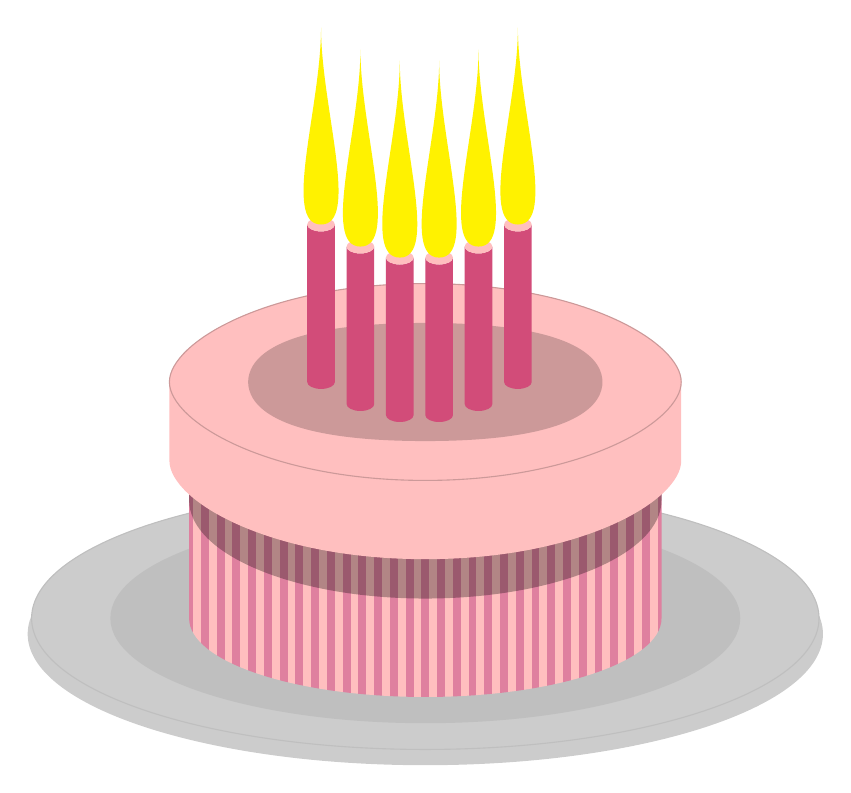
\begin{tikzpicture}
  \fill[white!80!black] (3,-.2) circle[x radius=5.05,y radius=1.66666];
  \fill[white!80!black] (3,0) circle[x radius=5,y radius=1.66666];
  \draw[white!75!black] (3,0) circle[x radius=5,y radius=1.66666];
  \fill[white!75!black] (3,0) circle[x radius=4,y radius=1.33333];
  \begin{scope}
    \clip (0,0) arc[x radius=3,y radius=1,start angle=180,delta angle=180]
       -- ++(0,2)  arc[x radius=3,y radius=1,start angle=0,delta angle=-180]
       -- ++(0,-2);
    \foreach \k in {0,...,60} {
      \pgfmathparse{Mod(\k,2) ? "pink" : "purple!50"}
      \let\linecol=\pgfmathresult
      \draw[line width=1mm,\linecol] (\k mm,2) -- ++(0,-3);
    }
  \end{scope}
  \fill[opacity=.3] (0,2)
    arc[x radius=3,y radius=1,start angle=180,delta angle=180] -- ++(0,-.5)
    arc[x radius=3,y radius=1.25,start angle=0,delta angle=-180] -- ++(0,.5);
  \fill[pink] (-.25,2) .. controls +(0,-.5) and +(-2,0) .. ++(3.25,-1.25)
    .. controls +(2,0) and +(0,-.5) .. ++(3.25,1.25) -- ++(0,1)
    .. controls +(0,.5) and +(2,0) .. ++(-3.25,1.25)
    .. controls +(-2,0) and +(0,.5) .. ++(-3.25,-1.25);
  \draw[pink!80!black] (-.25,3) .. controls +(0,-.5) and +(-2,0)
    .. ++(3.25,-1.25) .. controls +(2,0) and +(0,-.5) .. ++(3.25,1.25)
    .. controls +(0,.5) and +(2,0) .. ++(-3.25,1.25)
    .. controls +(-2,0) and +(0,.5) .. ++(-3.25,-1.25);
  \fill[pink!80!black] (.75,3) .. controls +(0,-.25) and +(-2,0)
    .. ++(2.25,-.75) .. controls +(2,0) and +(0,-.25) .. ++(2.25,.75)
    .. controls +(0,.25) and +(2,0) .. ++(-2.25,.75)
    .. controls +(-2,0) and +(0,.25) .. ++(-2.25,-.75);
  \foreach \i in {0,...,5} {
    \pgfmathsetmacro{\yshift}{-\i * (5 - \i) * .07cm}
    \begin{scope}[xshift=\i * .5cm,yshift = \yshift]
      \fill[purple!70] (1.5,3) arc[x radius=5pt, y radius=2.5pt,
        start angle=-180, end angle=0] -- ++(0,2) arc[x radius=5pt,
        y radius=2.5pt, start angle=0, end angle=-180] -- cycle;
      \fill[pink] (1.5,5) arc[x radius=5pt, y radius=2.5pt,
        start angle=-180, end angle=180];
      \fill[yellow] (1.5,7.5) ++(5pt,0) .. controls +(0,-1) and +(.5,0)
        .. ++(0,-2.5) .. controls +(-.5,0) and +(0,-1) .. ++(0,2.5);
    \end{scope}
  }
\end{tikzpicture}
\end{document}
